% Manuscript A -- PLOS ONE Research Article.
% Built on the PLOS ONE LaTeX template (article class), rebuilt by hand.
% Figures are NOT embedded in this file (PLOS policy); figure files are in figures/.
% For a reading copy with the figure embedded, build main_preview.tex.
\documentclass[10pt,letterpaper]{article}
\usepackage[top=0.85in,left=2.75in,footskip=0.75in]{geometry}

% amsmath and amssymb packages, useful for mathematical formulas and symbols
\usepackage{amsmath,amssymb}

% Use adjustwidth environment to exceed column width (see tables)
\usepackage{changepage}

% Input encoding and additional characters
\usepackage[utf8]{inputenc}
\usepackage{textcomp,marvosym}

% cite package, to clean up citations in the main text. Do not remove.
\usepackage{cite}

% nameref and hyperref (links hidden)
\usepackage{nameref,hyperref}
\hypersetup{hidelinks}

% line numbers
\usepackage[right]{lineno}

% ligatures disabled
\usepackage[nopatch=eqnum]{microtype}
\DisableLigatures[f]{encoding = *, family = * }

% tables
\usepackage{array}
\usepackage{booktabs}

% graphics are used only in the preview build
\usepackage{graphicx}
\newif\ifpreview
\ifdefined\PreviewMode\previewtrue\fi

% Text layout
\raggedright
\setlength{\parindent}{0.5cm}
\textwidth 5.25in
\textheight 8.75in

% Bold the 'Fig #' in the caption and separate it from the title/caption with a period
% Captions will be left justified
\usepackage[aboveskip=1pt,labelfont=bf,labelsep=period,justification=raggedright,singlelinecheck=off]{caption}
\renewcommand{\figurename}{Fig}

% References: Vancouver numbered style for review (plos2015.bst at acceptance; see README.md)
\bibliographystyle{vancouver}

% Remove brackets from numbering in List of References
\makeatletter
\renewcommand{\@biblabel}[1]{\quad#1.}
\makeatother

% Header and footer
\usepackage{lastpage,fancyhdr}
\pagestyle{fancy}
\fancyhf{}
\rfoot{\thepage/\pageref{LastPage}}
\renewcommand{\headrulewidth}{0pt}
\renewcommand{\footrule}{\hrule height 2pt \vspace{2mm}}
\fancyheadoffset[L]{2.25in}
\fancyfootoffset[L]{2.25in}
\lfoot{\today}

%% Macros
\newcommand{\Eq}[1]{Eq~(\ref{#1})}
\newcommand{\dt}{\Delta\tau}
%% END MACROS SECTION

\begin{document}
\vspace*{0.2in}

\begin{flushleft}
{\Large
\textbf\newline{Allowance edges or transfer edges? Evaluating on-chain wallet reputation out of window against degree baselines}
}
\newline
\\
Taehong Kwon\textsuperscript{1*},
Ernest Mnkandla\textsuperscript{1},
Donatien Koulla Moulla\textsuperscript{2},
David Sena Attipoe\textsuperscript{3}
\\
\bigskip
\textbf{1} School of Computing, College of Science, Engineering and Technology, University of South Africa, [city to be confirmed], South Africa
\\
\textbf{2} [affiliation to be confirmed]
\\
\textbf{3} [affiliation to be confirmed]
\\
\bigskip

* thkwon@enu-tech.co.kr

\end{flushleft}

% Please keep the abstract below 300 words
\section*{Abstract}
Lending and margin protocols that deal with pseudonymous counterparties have proposed ranking addresses by their public ledger activity. The established graph method runs PageRank over token transfers, yet a transfer only records a payment, whereas an ERC-20 allowance records an owner authorizing a spender to move its tokens. We ask what the allowance edge adds. PageRank on the latest allowances (EndorseRank) is compared with the transfer-based Adaptive Weighted PageRank (AWP) and with the raw degree counts that both walks smooth, on Arbitrum One logs drawn around 5,521 traders of a perpetual futures exchange; most ranked addresses are contracts. Scores are frozen before two three-month label windows, the second extracted only after a companion study's registration had fixed its cohorts and labels. Allowance scores track which spenders later gain new approvals and transfer scores which gain new senders, yet in neither window does any PageRank match the raw degree of its own edge type on that edge type's own construct (Kendall rank correlation on new approvals: count 0.711, EndorseRank 0.394). On this one-hop sample EndorseRank equals a common constant times one plus the damped owner-normalized in-strength, so multi-hop propagation remains untested. On trader outcomes, a post hoc analysis, planned after the June--August single-score results and hence the point estimates of both decision contrasts were known, found that having received any approval (44 and 39 traders) ranked later avoidance of forced liquidation above the transfer in-degree, with 97.5\% intervals, the Bonferroni level of the decision pair, above zero in both windows, which largely re-observe the same recipients. The like-for-like PageRank pair was not resolved. Nearly all recipients were contracts, a confound this design cannot assess; the signal was lower on the share of profitable closes and was not compared with traders' own liquidation histories.

\linenumbers

%======================================================================
\section*{Introduction}

Decentralized finance (DeFi) protocols lend, make markets and offer leveraged trading through smart contracts on public blockchains, with no custodian between the parties~\cite{schar2021,werner2022}. Their counterparties are pseudonymous addresses, which cost almost nothing to create and of which one operator may hold many~\cite{douceur2002}, so the identity checks and credit files of unsecured lending are unavailable~\cite{packin2024}. Protocols rely instead on over-collateralization and automatic liquidation~\cite{gudgeon2020crisis,bartoletti2021,perez2021}. A long-standing proposal is to let the ledger supply the missing history: a score computed from an address's public interactions could help a protocol screen counterparties or tier its risk parameters~\cite{do2023pagerank,lin2025riskprop,hassija2020,kotb2023}.

Graph ranking is the obvious instrument for such a score. PageRank gives every node the stationary probability of a damped random walk along directed edges~\cite{page1998,langville2006}, and EigenTrust and TrustRank adapt that walk to peer-to-peer networks and to web spam~\cite{kamvar2003,gyongyi2004trustrank}. On account-based ledgers the edges have so far been payments. Do and Do run PageRank and HodgeRank on Ethereum transactions as a measure of social credit~\cite{do2023pagerank}. The Adaptive Weighted PageRank (AWP) of Do, Do and Nguyen weights every transfer by a function that saturates in its value and decays logistically with its age, and restarts the walk at recently active senders~\cite{do2023awp}. Its authors validate AWP by its agreement with the number and value of transfers each address receives, statistics computed from the very transfers that make up its graph.

A transfer shows that value moved, not that the sender vouched for the recipient; routing contracts, market makers, airdrop hunters and wash traders all produce transfers in bulk~\cite{cong2023,luo2025}. The ERC-20 token standard records a second relation. By calling \texttt{approve}, or by signing an EIP-2612 \texttt{permit}, the holder of a token (the owner) lets another address (the spender) move up to a stated amount of the holder's balance~\cite{eip20,eip2612}. The resulting allowance is a standing capability until it is used up or revoked, and unlimited allowances, the majority of approvals on Ethereum, expose an owner's entire balance~\cite{wang2022}. A new approval for the same owner, spender and token overwrites the old one, so the latest allowance summarizes the relationship, and approvals are far rarer than transfers. Approvals have been used to link addresses controlled by one entity~\cite{victor2020}, but we know of no reputation method that ranks addresses on them.

An allowance is an authorization, and whether it also expresses trust is a question for the data. Most approvals are functional: to trade on an exchange a user must first approve its router or vault, whatever the user thinks of it. Approvals are also a route to theft, since a malicious or compromised spender can move every allowance it holds~\cite{wang2022}. What separates the allowance from the transfer is narrower: the holder of the funds grants it to one named spender, and it stays in force until it is spent or withdrawn. We therefore call the edge an authorization and keep the name EndorseRank only as the label of a method.

Whether either edge yields the better reputation score is partly a question of evaluation design, and two habits of the field make it hard to answer. One is to check a score against statistics of its own edges, an agreement that is expected by construction and speaks to the coherence of a construct, not to what else the score can tell us~\cite{cronbach1955,messick1995}. The other is to compare walks only with other walks. A PageRank smooths a local count, and local counts predict well: new links attach preferentially to nodes that already have many~\cite{barabasi1999,newman2001}, degree is a standard link-prediction baseline~\cite{libennowell2007}, also on Ethereum~\cite{lin2022linkpred}, and where degree correlations are weak PageRank is on average proportional to in-degree~\cite{fortunato2008}. A propagated score earns its extra cost only if it beats the count underneath it.

This paper compares authorization and payment edges with designs that address both habits. We compute EndorseRank, PageRank on the latest-allowance graph with AWP's edge weights and uniform restarts, alongside AWP and the two raw in-degrees on one sample of Arbitrum One addresses, freeze every score and test it on what happens afterwards, in two windows. Most addresses that receive approvals, and so most of those that EndorseRank can order, are contracts such as routers and vaults rather than the wallets of individual users. There are three contributions.

\begin{itemize}
\item An exact expression, up to a common constant, for EndorseRank on the depth-one allowance graphs that one-hop extraction yields. On such graphs the walk is a reweighted approval count, which confines any statement about propagation to graphs of this kind.
\item An out-of-window evaluation against the raw degrees in two windows. Each edge type's scores track later edges of the same type, a persistence check that motivates the degree baselines; on the label of that construct, no walk matches the raw degree of the edge type it walks on.
\item A comparison of the two edge types on trader outcomes that neither graph contains, fixed in a plan before it was computed but after some of its inputs were known. Having received any approval ranked later avoidance of forced liquidation above the transfer in-degree; the like-for-like PageRank pair is unresolved, the signal rests on a few dozen mostly contract accounts, and it does not extend to trading success.
\end{itemize}

\noindent A companion manuscript by the same authors (submitted to \textit{IEEE Access}; unpublished) studies a walk that mixes the two edge types, in the spirit of multilayer ranking~\cite{halu2013,dedomenico2015}, and its registered test, whose decision rule was not met. Both papers use the same extraction and June--August registration. The spender coefficients of the counts, AWP and EndorseRank, the runtimes and, briefly, the closed form appear in both; the trader comparison is reported here, apart from one decomposition of the mixed walk's trader result that the companion manuscript takes from it.

\subsection*{Related work}

\textit{On-chain reputation and risk.} Besides the two PageRank studies above~\cite{do2023pagerank,do2023awp}, RiskProp rates Ethereum accounts by spreading risk through the transaction network~\cite{lin2025riskprop}, and network embeddings of the transaction graph help detect phishing addresses~\cite{wu2022phishers}. Surveys of blockchain trust and reputation systems find explicit ratings and transfer volume to be the usual signals~\cite{bellini2020,almasoud2020}. Decentralized credit-scoring designs combine ledger records with prospect theory~\cite{hassija2020} or machine learning~\cite{kotb2023}, and legal scholarship warns that such scores can become as opaque as the models they would replace~\cite{packin2024}. Human Passport weighs credentials, among them identity checks and on-chain history, to decide whether an address belongs to a distinct person~\cite{passport}; it gates addresses rather than ordering them by their relations. None of these approaches ranks addresses on ERC-20 allowances.

\textit{Trust propagation and its weak points.} HITS separates hubs from authorities~\cite{kleinberg1999}. EigenTrust normalizes local trust so that no peer can raise its own standing at will~\cite{kamvar2003}, and TrustRank lets trust flow outward from a vetted seed set~\cite{gyongyi2004trustrank}. Under uniform teleportation that protection is weaker. Link farms and alliances of farms can lift a target's PageRank~\cite{gyongyi2005alliances}, and symmetric reputation functions such as PageRank cannot be Sybil-proof, whereas certain asymmetric functions built on flows from a trusted node can~\cite{cheng2005}. Both results apply to allowance graphs, where an approval costs a transaction fee but locks no tokens.

\textit{Approvals.} EIP-20 specifies the allowance mechanism and EIP-2612 extends it to signed approvals~\cite{eip20,eip2612}. Wang et al.\ measure how common unlimited approvals are and how much value they expose~\cite{wang2022}, and Victor's self-authorization heuristic uses approvals to cluster addresses of one entity~\cite{victor2020}.

\textit{Baselines and evaluation.} Degree is the natural benchmark for predicting new links~\cite{barabasi1999,newman2001,libennowell2007,lin2022linkpred}, and PageRank often behaves like a monotone function of in-degree~\cite{fortunato2008}. Construct validity~\cite{cronbach1955,messick1995} separates what a score measures from its agreement with checks built into it. Writing down an analysis plan before results are seen, also for data that already exist, limits analytic flexibility~\cite{nosek2018}; we follow that practice for the trader comparison and state what was known when the plan was written.

%======================================================================
\section*{Materials and methods}

\subsection*{Data and cohorts}

All events come from Arbitrum One, an optimistic rollup on Ethereum~\cite{kalodner2018}, read from the public BigQuery table \texttt{goog\_blockchain\_arbitrum\_one\_us.logs} (project \texttt{bigquery-public-data}). Every cohort is drawn from one seed cohort of 5,521 wallets: every address that closed at least three positions on GMX~V2, a perpetual futures exchange on Arbitrum One~\cite{gmxdocs}, between 1~December~2025 and 31~May~2026. A close is one \texttt{PositionDecrease} event, so partial closes and liquidations both count (S1 Text gives contracts, events, fields and formulas). The list came from GMX events alone and was fixed before any approval or transfer was extracted, so membership does not depend on either graph; but because it counts closes up to 31~May~2026, it also selects on trading inside the spring label window defined below.

We extracted every ERC-20 \texttt{Approval} log in which a seed wallet is owner or spender and every \texttt{Transfer} log in which it is sender or recipient, with amounts in raw base units, unadjusted for decimals. Logs of non-fungible tokens share the signatures but carry no amount; they decode to zero and were dropped with zero-value transfers. For each owner, spender and token only the most recent approval, in block and log order, is kept, and a latest value of zero removes the entry. The full scoring window holds 21,585 latest allowances, 13,055 (60.5\%) of them unlimited, close to the share reported for Ethereum~\cite{wang2022}. Two unmeasured properties of the event limit how directly a latest allowance records a fresh grant: some tokens also emit it when \texttt{transferFrom} spends a finite allowance, and contracts such as Uniswap's Permit2 keep inner allowances in differently signed events that we did not read (S1 Text). Because an event is kept only when a seed wallet takes part in it, every graph is the one-hop ego network of the seed cohort and an edge between two outside addresses is never observed, which, as Results show, decides what the allowance walk can compute.

Two kinds of addresses are scored after a freeze date. EndorseRank ranks the receiving side of an approval, and owners that receive no approval all share one value, so its natural unit of analysis is the spender. A spender cohort therefore holds every address with at least one positive latest allowance at the freeze. A trader cohort holds the seed wallets that are present in the graphs at the freeze and that closed at least three GMX positions in the subsequent label window, a rule that uses the label window. Traders with an in-approve degree above zero at the freeze are called recipients.

Account types were read with \texttt{eth\_getCode} at block 510,408,687, at the end of September 2026 and so after both label windows, for the 1,335 spring spenders: 1,174 held contract code and 161 were externally owned accounts (EOAs), one of them delegating to contract code under EIP-7702 and counted as an EOA (S1 Text). All 100 spenders that EndorseRank ranks highest in the spring are contracts, as are 221 of the 222 that gained a new approval pair. Recipient traders take their type from this lookup, or are unknown if they were not spring spenders; traders without approvals were never classified.

The study uses two windows (S1 Table). In the spring window (W0) scores use events from 1~December~2025 to 28~February~2026 (23:59:59~UTC), labels are counted from 1~March to 31~May~2026, and the cohorts hold 1,335 spenders and 1,860 traders, the latter out of 4,227 seed wallets present in the freeze-date graphs. In W1 scores use events from 1~December~2025 to 31~May~2026, labels are counted from 1~June to 31~August~2026, and the cohorts hold 1,964 spenders and 1,402 traders, out of 5,151 seed wallets present at the freeze. The windows are not independent samples: W1's scoring window contains W0's scoring and label windows, and many addresses belong to the cohorts of both. The June--August logs (163,553 approvals, 1,013,023 transfers and 144,152 GMX closes) were extracted on 1~October~2026, after a registration committed that day for the companion study had fixed its cohorts, labels, queries and code, a gate the extraction script enforces. AWP and the two counts were among the scores of that registered evaluation; EndorseRank was scored on the W1 cohorts afterwards, and no comparison in this paper is registered. W1 is data extracted after the patterns below were first seen in the spring.

\subsection*{Scores}

\subsubsection*{Weighted PageRank}
Every score is computed by one weighted PageRank solver. With edge weights $w(u,v)$, out-strength $o(u)=\sum_v w(u,v)$ and a restart distribution $\boldsymbol{\pi}$ over the node set $V$, the iteration is
\begin{equation}
\label{eq:pagerank}
\mathbf{r}^{(t+1)} = (1-d)\,\boldsymbol{\pi} + d\,P^{\top}\mathbf{r}^{(t)} + d\,\Bigl(\sum_{u:\,o(u)=0} r^{(t)}_u\Bigr)\boldsymbol{\pi},
\qquad
P_{uv}=\frac{w(u,v)}{o(u)}\ \text{if } o(u)>0,
\end{equation}
where the rows of dangling nodes ($o(u)=0$) are zero, so that the last term returns their mass through $\boldsymbol{\pi}$. The damping factor is $d=0.85$, the iteration starts from the uniform vector, and it stops once the $L_1$ change falls below $10^{-8}$ or after 300 iterations. A seed wallet that a graph does not contain scores zero under that graph's methods, as the plan for the trader comparison also fixed.

\subsubsection*{AWP on transfers}
Following Do, Do and Nguyen~\cite{do2023awp}, a transfer $e$ of amount $x_e$ made $\Delta t_e$ days before the decay anchor adds $\sigma(\Delta t_e)\,V(x_e)$ to the edge from its sender to its recipient, with
\begin{equation}
\label{eq:weights}
\sigma(\Delta t)=\frac{1}{1+\exp\bigl(k(\Delta t-t_0)\bigr)},
\qquad
V(z)=\frac{2}{1+e^{-bz}}-1,
\end{equation}
so that
\begin{equation}
\label{eq:awp-weight}
w_T(u,v)=\sum_{e:\,u\to v}\sigma(\Delta t_e)\,V(x_e),
\qquad
\pi_u\propto X_u=\sum_{v\neq u}\ \max_{e:\,u\to v}\sigma(\Delta t_e).
\end{equation}
The restart weight $X_u$, which the authors call activeness, sums the time weight of $u$'s latest transfer to each address it has paid. We found no parameter values in the paper; $k=0.01$, $t_0=180$ days and $b=1$ on raw base units are our choices. With $b=1$, $V(x_e)$ lies within $10^{-4}$ of one for the 99.5\% of transfers of ten base units or more, so AWP's value weighting is in effect switched off and an edge weight is an age-discounted count of transfers. Every statement about AWP below concerns this variant; value weights on decimal-adjusted or price-normalized amounts were not tried and might serve AWP better. The time discount runs from $\sigma(0)=0.858$ to $\sigma(182)=0.495$.

\subsubsection*{EndorseRank on latest allowances}
EndorseRank puts AWP's weights on the allowance graph. An edge $u\to v$ means that owner $u$ holds a positive latest allowance for spender $v$ on at least one token, and its weight is
\begin{equation}
\label{eq:er-weight}
w_A(u,v)=\sum_{\mathrm{token}}\sigma\bigl(\Delta t^{\star}(u,v,\mathrm{token})\bigr)\,V\bigl(a^{\star}(u,v,\mathrm{token})\bigr),
\end{equation}
where $a^{\star}$ is the latest allowance and $\Delta t^{\star}$ the age of the approval that set it. Because 99.9\% of allowances exceed ten base units, $w_A(u,v)$ amounts to a count of the tokens for which $u$ has approved $v$, discounted by age, and an unlimited allowance weighs no more than a small one. EndorseRank restarts uniformly. AWP's restart rule, transplanted to allowances, would send restart mass to owners in proportion to how many spenders they had recently approved, rewarding the granting of approvals rather than their receipt. We adopted the uniform rule after scoring both rules on these data, and so also report EndorseRank with activity restarts, which shares AWP's weights and restart rule and differs from AWP only in its edges: AWP's like-for-like PageRank counterpart.

\subsubsection*{Raw degrees}
The in-approve degree of an address is the number of distinct owners that hold a positive latest allowance for it, and its transfer in-degree is the number of distinct other addresses that have sent it a transfer, both counted at the freeze:
\begin{equation}
\label{eq:degrees}
k_A(v)=\bigl|\{u : a^{\star}(u,v,\cdot)>0\}\bigr|,
\qquad
k_T(v)=\bigl|\{u\neq v : u \text{ sent a transfer to } v\}\bigr|.
\end{equation}
Each count is the local statistic that one of the two PageRanks smooths, and out of window each serves as the baseline that its PageRank has to beat. The decay of \Eq{eq:weights} is anchored at the freeze date; in W0 all ages are below 90 days and the time weights lie between about 0.71 and 0.86.

\subsection*{Labels}

\textit{Spender labels.} Two counts are taken in the label window, one per construct: authorization adoption, how many new owners come to authorize a spender, and payment inflow, how many new addresses start paying it. Both describe how counterparties take up an address, but both count edges of the kinds that build the graphs, so agreement with them shows persistence rather than anticipation of a different outcome. New approval pairs counts the owners that give the spender a positive approval in the window while their pair held no positive latest allowance at the freeze. New transfer senders counts the distinct addresses that send the spender a transfer in the window without having sent it one since 1~December~2025, self-transfers excluded. Both labels are sparse. In W0, 222 of the 1,335 spenders gained a new approval pair and 175 a new sender; in W1, 158 and 136 of the 1,964 did.

\textit{Trader labels.} Six outcomes are computed from each trader's GMX closes in the label window, for traders with at least three closes there (formulas in S1 Text). A close is a liquidation when the event marks it as a liquidation order or it was executed through the exchange's liquidation handler. The liquidation-free close rate (LFCR) is one minus the share of closes that ended in liquidation, and the no-liquidation flag is one when none did. The number of profitable closes and the realized gain, the sum of positive profits, grow with the amount of trading; the profitable share and the non-loss share of closes do not. Profits are the profit-or-loss field of each close event as recorded, with separately reported fees not deducted. Two details matter below. Partial closes count as closes, so a trader who reduces positions in steps has more closes per liquidation, and a higher LFCR, than one who closes at once. And a liquidated close is neither profitable nor losing, so it lowers the profitable share but raises the non-loss share. In W1, 789 of the 1,402 traders had at least one liquidation and 17 had every close liquidated; in W0, 923 of the 1,860 had at least one.

The six outcomes come from the exchange's position events, not from the edges of either graph; in that sense we call them outcomes built from neither edge type. They are not wholly separate from the transfer layer, though: the exchange settles collateral and profits in ERC-20 tokens, so past payouts also appear as transfers in the pre-freeze transfer graph.

A liquidation happens when the collateral behind a leveraged position no longer covers its losses and the exchange closes the position~\cite{perez2021}. It is not a credit default, since the position is settled against the trader's own collateral, but among the outcomes in these data it comes nearest to a counterparty failing to cover its obligations. Being a rate, LFCR does not reward an address simply for trading more, although the chance of at least one liquidation still rises with the number of closes. LFCR was among the labels registered for W1 for the companion study.

\subsection*{Comparison plan for outcomes built from neither edge type}

The comparison of the two edge types on trader outcomes was fixed in a written plan, reproduced verbatim as S1 File and committed to the authors' repository on 9~October~2026 at 02:39~UTC (commit \texttt{20e250f}); the analysis script followed at 02:42 (\texttt{dbe7cf0}) and the results at 02:51 (\texttt{b89c48e}), git timestamps in the authors' own repository rather than independent ones. The plan preceded its decision contrasts and every stratified, recipient and spring-window result, but not all of its inputs, so it is a pre-specified post hoc analysis of existing data~\cite{nosek2018}. By then the W1 labels had been counted, and the W1 coefficients of the two counts and AWP on all six labels, and of both EndorseRank variants on LFCR, had been computed with 400 resamples. The W1 point estimates of P on every label and of Q on LFCR, defined below, were therefore implied by known numbers, and P was made a decision contrast with that knowledge. EndorseRank minus AWP on LFCR in W1 had itself been computed ($+0.035$, $[-0.017,0.087]$). No W0 association with a trader label had been computed, and one related number pointed against the allowance side: within the scoring window, LFCR had agreed slightly more with a walk over raw-amount transfers than with one over raw-amount allowances ($\tau=0.083$ against $0.075$).

The plan sets allowance-side scores against transfer-side scores in pairs. The decision contrasts on LFCR in W1 are P, the in-approve degree minus the transfer in-degree, and Q, EndorseRank with activity restarts minus AWP, the like-for-like PageRank pair. EndorseRank minus AWP and EndorseRank minus the in-approve degree are reported without entering a decision, as are all contrasts on the other five labels and everything in W0. The plan also contains three contrasts involving walks over raw-amount layers that belong to the companion study; S2 Table lists them with every other row, and the text does not discuss them. Three rules were fixed in advance.
\begin{itemize}
\item R1, a count-level lead on liquidation avoidance, holds if the 97.5\% interval of P lies above zero in W1, the 95\% interval of P stratified by the number of closes lies above zero in W1, the point estimate of P is positive in W0, and, if at least 30 recipients are EOAs, P restricted to them is positive.
\item R2, a PageRank-level lead, holds if the 97.5\% interval of Q lies above zero in W1 and the point estimate of Q is positive in W0.
\item R3 applies if P on the profitable share or on the non-loss share in W1 is negative with a 95\% interval that excludes zero; the allowance signal is then to be read as specific to liquidation avoidance and as running against loss avoidance.
\end{itemize}
Recipients are compared with all other labelled traders on their liquidation record, outcome means and number of closes. An influence check recomputes P without the ten recipients of highest in-approve degree. The plan does not say how ties are broken; the script sorts with the default sort of the pandas library, which does not preserve the input order of equal values, so when nearly every recipient has degree one the ten dropped are in effect arbitrary.

\subsection*{Order of the analyses}

Because the analyses were fixed at different times relative to the data, their order is stated here. (i) Every spring spender contrast was computed after the spring labels were known and is exploratory. (ii) EndorseRank's uniform restart rule was chosen after both rules had been scored on the spring data. (iii) On 1~October~2026 the June--August design was registered for the companion study and its logs extracted; EndorseRank was scored after that registered evaluation. (iv) On 9~October~2026 the trader plan was committed; its decision contrasts, the 2,000-resample intervals and all spring-window liquidation associations were computed afterwards. (v) The closed form was derived after all out-of-window results were known; it is an analytic account of them, not a further test.

\subsection*{Statistical analysis}

Agreement between a score and a label is measured by Kendall's rank correlation~\cite{kendall1938}, in its tie-corrected form $\tau_b$, on raw scores and raw label values, so that tied scores stay tied. We write $\tau(a)$ for the coefficient of score $a$ and $\dt=\tau(a)-\tau(b)$ for a paired contrast. Uncertainty comes from a paired wallet bootstrap~\cite{efron1979} with percentile intervals~\cite{diciccio1996}: wallets are resampled with replacement, and one matrix of resample indices is shared by every score, so a contrast keeps the covariance of its two scores. The intervals treat wallets as independent and the graphs, and so the scores, as fixed; they ignore that spenders share owners and recipients may share contract code. The spender holdouts use 400 resamples with seed 42, the trader comparison 2,000 with the same seed. Only the decision pair $\{\mathrm{P},\mathrm{Q}\}$ in W1 is judged on Bonferroni-adjusted 97.5\% intervals; every other interval, including the 97.5\% intervals shown for W0, is unadjusted and descriptive. A contrast is described as a difference when its interval excludes zero. No $p$-values are reported, and no causal claim is made.

Two properties of $\tau_b$ bear on the comparisons. Its tie correction treats a predictor with few distinct values differently from a nearly tie-free one, so part of a gap between a heavily tied count and a walk that breaks its ties may reflect ties rather than information. And a rare indicator, as the in-approve degree is among traders, can reach only a $\tau_b$ far below one, so a difference in $\tau_b$ mixes prevalence with association; we therefore also describe the trader result by the difference in no-liquidation rates between recipients and other traders. Because a trader who closes more positions has more chances to be liquidated at least once, $\tau_b$ is additionally calculated within groups of 3--4, 5--9, 10--24 and at least 25 closes in the label window and averaged with weights proportional to the number of wallet pairs per group. The number of closes is measured after the freeze, so this stratification is descriptive.

\subsection*{Closed-form check and runtime}

The closed form derived in Results was checked against EndorseRank as computed on the allowance graphs at both freezes, with self-loops removed for the check: for every spender we computed its relative error, and over all spenders the Spearman correlation of EndorseRank with the owner-normalized in-strength and with the in-approve degree. Runtime covers one solver call on prebuilt edge lists, matrix assembly and power iteration included: one untimed warm-up and five timed runs of one Python implementation (SciPy sparse matrices, NumPy power iteration) with identical settings, in a cloud container with four cores of a 2.8\,GHz Intel Xeon processor and 15\,GB of memory (Python~3.11, NumPy~2.4, SciPy~1.17).

\subsection*{Ethics statement}

This study used only publicly available blockchain data and involved no human participants. No attempt was made to link any address to a real-world identity, and only aggregate statistics are reported. [ethics clearance reference to be added by the authors]

\subsection*{Data availability}

The evaluation code, the versioned configuration, the SQL queries, the extraction manifests, the machine-readable summaries behind every table, the registration files of the June--August window, the analysis plan, script and results of the trader comparison, and the per-wallet analysis frames are held in two Git repositories of the authors, which are currently private: \nolinkurl{github.com/abitocodes/phd_works}, folder \nolinkurl{1-Dissertation-Works/ERC20-Allowance-PageRank-Wallet-Reputation/dissertation/wallet-reputation-experiments} (registration commit \texttt{4085ab9}, table revision \texttt{7129981}), and \nolinkurl{github.com/abitocodes/phd-dissertation-draft-en}, folder \nolinkurl{analysis/} (plan \texttt{20e250f}, script \texttt{dbe7cf0}, results \texttt{b89c48e}). Both will be made public, with an archived release, before submission [archive DOI, and an anonymous reviewer link if the release is delayed, to be inserted by the authors]. The plan is also S1 File, and the queries are in S1 Text. The raw logs can be re-extracted from the public BigQuery table named above; because that table is not a versioned snapshot, the archive will also hold the extracted log subsets, or their hashes, with the query text and run dates. [How addresses in the per-wallet frames are deposited is to be decided by the authors, consistently with the Ethics statement.]

\subsection*{Use of generative AI}

Claude (Anthropic), used through the Claude Code agent, was used in this study for more than language editing. In the repository that holds the trader comparison, the tool drafted the analysis plan (S1 File, commit \texttt{20e250f}), wrote and ran the analysis script and the closed-form check (commits \texttt{dbe7cf0} and \texttt{cde51b8}), and produced the results files and the tables derived from them (\texttt{b89c48e}); these commits carry the author name Claude. The tool also generated Fig 1 and S1 and S2 Tables from those results, drafted and revised the text of this manuscript, its supporting information and the cover letter, and checked text and analysis scripts for errors. [The authors to state any further use, for example in the evaluation pipeline, and how they verified the tool's outputs, for instance by an independent re-run of the analysis scripts, review of the code, or a check of each reported number against the results files.] The authors take full responsibility for the content of the article.

%======================================================================
\section*{Results}

\subsection*{Graph structure}

The allowance graph is nearly bipartite (Table~\ref{tab1}). At the W1 freeze it has 6,442 nodes and 14,727 edges, one a self-loop; 4,479 nodes have out-edges only (pure owners), 1,852 in-edges only (pure spenders) and just 111 both, and apart from the self-loop it has no cycle. The transfer graph over the same window has 30,791 nodes and 137,087 edges, a largest strongly connected component of 9,278 addresses (30\% of nodes), and 28.5\% of its edges reciprocated. Among the 5,521 seed wallets, 4,424 are owners that receive no approval and share one EndorseRank value, 966 are touched by no allowance edge and score zero, and only 131 rank above the common value, so EndorseRank says almost nothing about most traders and its out-of-window evaluation rests on spenders. Among the 1,335 spring spenders it leaves almost no ties (1,291 distinct values, largest tie block 42).

\begin{table}[!ht]
\centering
\caption{{\bf Allowance graphs at the two freeze dates and fit of the closed form for EndorseRank.}}
\begin{tabular}{lrr}
\toprule
 & W0 freeze & W1 freeze \\
 & 28 Feb 2026 & 31 May 2026 \\
\midrule
Nodes & 4,743 & 6,442 \\
Edges (self-loops removed) & 9,765 & 14,726 \\
Pure owners (out-edges only) & 3,408 & 4,479 \\
Pure spenders (in-edges only) & 1,243 & 1,852 \\
Nodes with in- and out-edges & 92 & 111 \\
Spenders with an in-neighbor that has in-edges & 50 & 58 \\
Common score $c$ of nodes without in-edges & $1.29\times10^{-4}$ & $9.62\times10^{-5}$ \\
\midrule
Spenders within 1\% of \Eq{eq:closed-form} & 96.4\% & 97.4\% \\
Median relative error of \Eq{eq:closed-form} & $4.8\times10^{-10}$ & $3.8\times10^{-10}$ \\
Spearman $\rho$, EndorseRank and $\delta$ & 0.945 & 0.980 \\
Spearman $\rho$, EndorseRank and in-approve degree & 0.584 & 0.568 \\
Spearman $\rho$, $\delta$ and in-approve degree & 0.589 & 0.570 \\
\bottomrule
\end{tabular}
\begin{flushleft}Graphs built from the latest allowances up to each freeze date, restricted to edges incident to the seed cohort. Spenders are the nodes with in-edges. $\delta$ is the owner-normalized in-strength of \Eq{eq:closed-form}. The W1 graph has one self-loop (14,727 edges with it), which the solver keeps and this check removes. The node that carries it has no other in-edge, so the table counts 1,963 nodes with in-edges against the 1,964 addresses of the W1 spender cohort.
\end{flushleft}
\label{tab1}
\end{table}

\subsection*{Each edge type tracks later edges of its own type}

Table~\ref{tab2} sets every score frozen at each date against the two spender labels. As persistence would lead one to expect, the edge type decides which label a score tracks. On new approval pairs in the spring window, the in-approve degree reaches $\tau=0.711$, EndorseRank $0.394$ and its activity-restart variant $0.372$, while AWP ($0.123$) and the transfer in-degree ($0.117$) stay low. The pattern repeats in W1 ($0.613$, $0.333$, $0.325$, $0.118$ and $0.128$). EndorseRank leads AWP on this label by $+0.271$ $[0.207,0.332]$ in W0 and $+0.215$ $[0.171,0.270]$ in W1. On new transfer senders the transfer in-degree leads ($0.472$ and $0.435$), and AWP is ahead of EndorseRank by $+0.061$ $[0.026,0.098]$ and $+0.064$ $[0.036,0.088]$. The two sides are not symmetric. Spenders that many owners approve also attract many new senders, so the in-approve degree ranks new senders fairly well ($0.404$ and $0.371$), whereas no transfer-side score ranks new approvals above $0.13$. These results describe contracts more than user wallets: all 100 spenders that EndorseRank ranks highest in the spring, and 221 of the 222 that gained a new approval pair, hold contract code.

\begin{table}[!ht]
\begin{adjustwidth}{-2.25in}{0in}
\centering
\caption{{\bf Spender holdouts: scores frozen at each date against labels counted over the next three months.}}
\footnotesize
\setlength{\tabcolsep}{4pt}
\begin{tabular}{lcccc}
\toprule
 & \multicolumn{2}{c}{W0: freeze 28 Feb 2026 ($n=1{,}335$)} & \multicolumn{2}{c}{W1: freeze 31 May 2026 ($n=1{,}964$)} \\
\cmidrule(lr){2-3}\cmidrule(lr){4-5}
Score at the freeze & New approval pairs & New senders & New approval pairs & New senders \\
\midrule
In-approve degree (count) & 0.711 [0.665, 0.759] & 0.404 [0.348, 0.467] & 0.613 [0.564, 0.663] & 0.371 [0.313, 0.429] \\
Transfer in-degree (count) & 0.117 [0.049, 0.191] & 0.472 [0.423, 0.520] & 0.128 [0.064, 0.188] & 0.435 [0.401, 0.468] \\
EndorseRank & 0.394 [0.360, 0.431] & 0.283 [0.247, 0.320] & 0.333 [0.306, 0.364] & 0.255 [0.227, 0.284] \\
EndorseRank, activity restarts & 0.372 [0.327, 0.417] & 0.301 [0.254, 0.348] & 0.325 [0.295, 0.358] & 0.284 [0.252, 0.312] \\
AWP & 0.123 [0.068, 0.177] & 0.344 [0.307, 0.383] & 0.118 [0.071, 0.161] & 0.319 [0.291, 0.345] \\
\midrule
\multicolumn{5}{l}{\emph{Paired differences, $\dt$ [95\% CI]}} \\
EndorseRank $-$ in-approve degree & $-0.317$ [$-0.354$, $-0.283$] & & $-0.280$ [$-0.313$, $-0.247$] & \\
AWP $-$ transfer in-degree & & $-0.127$ [$-0.150$, $-0.099$] & & $-0.116$ [$-0.133$, $-0.095$] \\
EndorseRank $-$ AWP & $+0.271$ [0.207, 0.332] & & $+0.215$ [0.171, 0.270] & \\
AWP $-$ EndorseRank & & $+0.061$ [0.026, 0.098] & & $+0.064$ [0.036, 0.088] \\
\bottomrule
\end{tabular}
\begin{flushleft}Kendall $\tau_b$ with 95\% percentile interval from 400 paired wallet resamples (seed 42); intervals are unadjusted and descriptive. Spenders hold at least one positive latest allowance at the freeze. In W0, 222 gained at least one new approval pair and 175 at least one new sender; in W1, 158 and 136 did. None of these contrasts was fixed before the spring labels were known, and in W1 EndorseRank was scored after the registered evaluation.
\end{flushleft}
\label{tab2}
\end{adjustwidth}
\end{table}

\subsection*{No PageRank beats the raw degree of its own edge type}

The second pattern in Table~\ref{tab2} is that, on the label of its own construct, every walk falls short of the count it smooths. EndorseRank minus the in-approve degree on new approval pairs is $\dt=-0.317$ $[-0.354,-0.283]$ in W0 and $-0.280$ $[-0.313,-0.247]$ in W1, and AWP minus the transfer in-degree on new senders is $-0.127$ $[-0.150,-0.099]$ and $-0.116$ $[-0.133,-0.095]$. Activity restarts do not rescue EndorseRank ($0.372$ and $0.325$ on new approval pairs). Off their own constructs the counts are not always ahead; on traders' profitable closes, for instance, EndorseRank ranks above the in-approve degree in both windows (S2 Table). Because most spenders have a single owner, the count is heavily tied while the walks are nearly tie-free, so part of these gaps may reflect how $\tau_b$ treats ties; no tie-robust comparison was made.

Coverage does not explain the shortfall. The 318 spring spenders with no transfer edge before the freeze score zero under AWP; they gained a new approval pair more often than the others (22\% against 15\%) and a new sender less often (4\% against 16\%). Among the 977 spenders with an incoming transfer from another address before the freeze, a restriction chosen after the results were known, AWP still trails the transfer in-degree on new senders ($0.388$ against $0.701$; $\dt=-0.314$ $[-0.353,-0.276]$), and EndorseRank trails the in-approve degree on new approval pairs ($0.340$ against $0.679$). A spender is more likely to gain new counterparties of a kind the more it already has, as preferential attachment would lead one to expect~\cite{barabasi1999,newman2001}, and the count records this directly; we did not estimate the form of that dependence. Both walks instead divide each endorser's or payer's weight among all the addresses it approves or pays.

\subsection*{What EndorseRank computes on a depth-one graph}

The one-hop extraction makes almost every node of the allowance graph either a pure owner or a pure spender (Table~\ref{tab1}). On a graph of that shape EndorseRank can be written out.

\textit{Observation.} Let PageRank follow \Eq{eq:pagerank} with damping $d$ and restart distribution $\boldsymbol{\pi}$, let $r_D$ be the total score of the dangling nodes, and write $C=1-d+d\,r_D$. Every node $u$ without in-edges then scores $r_u=C\pi_u$, and a node $v$ none of whose in-neighbors has an in-edge of its own scores $r_v=C\bigl(\pi_v+d\sum_u \pi_u\,w(u,v)/o(u)\bigr)$. With uniform restarts, $\pi_u=1/|V|$, all nodes without in-edges share the score
\begin{equation}
\label{eq:c}
c=\frac{1-d+d\,r_D}{|V|},
\end{equation}
and such a node $v$ scores
\begin{equation}
\label{eq:closed-form}
r_v=c\,\bigl(1+d\,\delta(v)\bigr),
\qquad
\delta(v)=\sum_{u}\frac{w(u,v)}{o(u)}.
\end{equation}
Here $\delta(v)$ is the owner-normalized in-strength of $v$: each owner $u$ contributes the share of its own approval weight that goes to $v$, so an owner that approves many spenders adds little to each of them.

\textit{Derivation.} At the fixed point of \Eq{eq:pagerank} every node $v$ receives $(1-d)\pi_v$ from teleportation and $d\,r_D\pi_v$ from the dangling rows, together $C\pi_v$, plus $d\sum_u r_u\,w(u,v)/o(u)$ from its in-neighbors. A node without in-edges receives only $C\pi_u$. If every in-neighbor $u$ of $v$ is such a node, substituting $r_u=C\pi_u$ gives the result, and \Eq{eq:closed-form} follows for uniform $\boldsymbol{\pi}$.

The observation is a one-step expansion of the fixed point rather than a closed form in the strict sense, because $c$ depends on $r_D$, which the whole score vector determines; but $c$ is common to all the spenders it covers, so EndorseRank orders them exactly as $\delta(v)$ does. It describes the computed scores closely (Table~\ref{tab1}): 96.4\% and 97.4\% of spenders lie within 1\% of \Eq{eq:closed-form}, with median relative errors below $10^{-9}$, and the rest have an in-neighbor that itself receives approvals. Over the spenders, EndorseRank has a Spearman correlation of $0.945$ and $0.980$ with $\delta$ but only $0.584$ and $0.568$ with the in-approve degree. For the activity-restart variant, which \Eq{eq:closed-form} does not cover, a pure spender approves nobody and has $\pi_v=0$, so its score is proportional to $\sum_u \pi_u\,w(u,v)/o(u)$, the same in-strength with each owner weighted by its approving activity.

Two consequences follow. First, on this sample EndorseRank is a reweighted approval count. It departs from the in-approve degree through its time weights, its token weights (an owner that approves a spender on several tokens adds more) and the normalization by each owner's total approval weight; which of the three, or how much of the tie structure, costs the walk its agreement with later approvals was not isolated. Second, every path is one step long. A spender collects its mass from owners whose scores are equal, so an endorser's identity matters only through how widely it approves, and the walk had nothing to propagate. The finding that propagation adds nothing to the count is therefore confined to depth-one samples; testing it more generally needs a sample that reaches two or more hops beyond the seed wallets. AWP, on the cyclic transfer graph, has no comparable closed form and also trails its count.

\subsection*{Outcomes built from neither edge type}

Every result in this subsection belongs to the pre-specified post hoc analysis described in Materials and methods; Table~\ref{tab3} gives the contrasts on the liquidation-free close rate.

\begin{table}[!ht]
\begin{adjustwidth}{-2.25in}{0in}
\centering
\caption{{\bf Allowance-side minus transfer-side scores on the later liquidation-free close rate of traders.}}
\begin{tabular}{lccccc}
\toprule
Contrast ($a-b$) & $\tau(a)$ & $\tau(b)$ & $\dt$ & 95\% CI & 97.5\% CI \\
\midrule
\multicolumn{6}{l}{\emph{W1: freeze 31 May 2026, labels June--August 2026 ($n=1{,}402$ traders)}} \\
P: in-approve degree $-$ transfer in-degree & $0.144$ & $-0.006$ & $+0.150$ & $[0.100,\,0.201]$ & $[0.091,\,0.209]$ \\
\quad P, stratified by closes & $0.155$ & $-0.025$ & $+0.180$ & $[0.125,\,0.244]$ & -- \\
Q: EndorseRank (activity restarts) $-$ AWP & $0.077$ & $0.045$ & $+0.032$ & $[-0.003,\,0.065]$ & $[-0.008,\,0.071]$ \\
\quad Q, stratified by closes & $0.064$ & $0.043$ & $+0.021$ & $[-0.016,\,0.057]$ & -- \\
EndorseRank $-$ AWP & $0.081$ & $0.045$ & $+0.035$ & $[-0.018,\,0.088]$ & -- \\
EndorseRank $-$ in-approve degree & $0.081$ & $0.144$ & $-0.063$ & $[-0.105,\,-0.022]$ & -- \\
\midrule
\multicolumn{6}{l}{\emph{W0: freeze 28 Feb 2026, labels March--May 2026 ($n=1{,}860$ traders)}} \\
P: in-approve degree $-$ transfer in-degree & $0.114$ & $-0.040$ & $+0.153$ & $[0.115,\,0.193]$ & $[0.108,\,0.198]$ \\
\quad P, stratified by closes & $0.128$ & $-0.024$ & $+0.152$ & $[0.108,\,0.195]$ & -- \\
Q: EndorseRank (activity restarts) $-$ AWP & $0.032$ & $-0.002$ & $+0.034$ & $[0.004,\,0.064]$ & $[-0.001,\,0.068]$ \\
\quad Q, stratified by closes & $0.063$ & $0.026$ & $+0.037$ & $[0.006,\,0.068]$ & -- \\
EndorseRank $-$ AWP & $0.010$ & $-0.002$ & $+0.012$ & $[-0.027,\,0.052]$ & -- \\
EndorseRank $-$ in-approve degree & $0.010$ & $0.114$ & $-0.103$ & $[-0.140,\,-0.065]$ & -- \\
\bottomrule
\end{tabular}
\begin{flushleft}Kendall $\tau_b$ of score $a$ and score $b$ on traders with at least three closes in the label window, and their difference. Paired wallet bootstrap with 2,000 resamples (seed 42). Only the 97.5\% intervals of P and Q in W1 are decision intervals (Bonferroni level of that pair); every other interval, including the 97.5\% intervals in W0, is unadjusted and descriptive. Stratified rows combine $\tau_b$ within strata of 3--4, 5--9, 10--24 and 25 or more closes, weighted by wallet pairs; the strata are measured after the freeze. Pre-specified post hoc analysis: the plan was committed after the W1 labels and single-score coefficients were known, and before the decision contrasts and the stratified, recipient and W0 results were computed (EndorseRank $-$ AWP in W1 had been computed earlier with 400 resamples). S2 Table lists every contrast of the plan.
\end{flushleft}
\label{tab3}
\end{adjustwidth}
\end{table}

\textit{Counts (R1 holds).} Among traders the in-approve degree is in effect an indicator: only 44 of the 1,402 traders in W1 and 39 of the 1,860 in W0, about 3\% and 2\%, had received any approval at the freeze, all from one owner except five W1 traders with two. P thus compares having received an approval with the transfer in-degree. In W1 the indicator ranks the later liquidation-free close rate at $\tau=0.144$ and the transfer in-degree at $-0.006$, essentially not at all; P is $+0.150$, with a Bonferroni-adjusted 97.5\% interval of $[0.091,0.209]$, and $+0.180$ $[0.125,0.244]$ stratified by the number of closes. In W0 P is $+0.153$ (97.5\% interval $[0.108,0.198]$), and $+0.152$ $[0.108,0.195]$ stratified. All conditions of R1 hold; the condition on EOA recipients applies only when at least 30 recipients are EOAs, and with one per window it did not apply. Because the indicator is rare, the no-liquidation rates given below describe the effect more directly than P.

\textit{PageRanks (R2 fails).} Q, EndorseRank with activity restarts minus AWP, is $+0.032$ in W1 and $+0.034$ in W0, with 97.5\% intervals $[-0.008,0.071]$ and $[-0.001,0.068]$ that reach below zero. The walks lean the same way as the counts, but the difference is not resolved at this precision: the W1 interval of Q is about 0.08 wide, so a difference below about 0.04 could not have been resolved (for P the figure is about 0.06). EndorseRank with uniform restarts against AWP is not resolved either ($+0.035$ $[-0.018,0.088]$ in W1, $+0.012$ $[-0.027,0.052]$ in W0). EndorseRank also falls below the in-approve degree on this label ($\dt=-0.063$ $[-0.105,-0.022]$ in W1 and $-0.103$ $[-0.140,-0.065]$ in W0), but this shortfall may owe to a rule of the plan. Traders absent from the allowance graph score zero, below every owner, so EndorseRank orders the traders without approvals by whether they appear in the graph at all, which the count does not. Keeping them as isolated nodes would remove that ordering; that sensitivity analysis was not run on these labels.

\textit{The other labels (R3 applies).} Fig~\ref{fig1} shows that the allowance side leads only on the two liquidation labels. On the no-liquidation flag P is $+0.259$ $[0.199,0.320]$ and Q $+0.075$ $[0.035,0.116]$ in W1, and both stay above zero in W0 ($+0.237$ $[0.192,0.286]$ and $+0.060$ $[0.026,0.095]$). These intervals are unadjusted, enter no decision and do not change R2. On the two labels that grow with activity, the number of profitable closes and the realized gain, the transfer side leads: in W1, P is $-0.194$ $[-0.247,-0.139]$ and $-0.107$ $[-0.160,-0.052]$, and Q is $-0.136$ $[-0.168,-0.101]$ and $-0.124$ $[-0.155,-0.092]$. On the two shares, which do not grow with activity, the in-approve degree ranks below the transfer in-degree: P is $-0.101$ $[-0.149,-0.047]$ on the profitable share and $-0.138$ $[-0.191,-0.083]$ on the non-loss share, and in W0 $-0.074$ $[-0.126,-0.016]$ and $-0.113$ $[-0.164,-0.060]$. R3 therefore applies. The non-loss share needs care: a liquidated close counts as not losing, so that share rises with liquidations by construction, and part of the negative P on it follows from the recipients' rarity of liquidation. The profitable share counts liquidated closes as unprofitable, which if anything favors the recipients, and there too they rank lower. The construct that the indicator ranks is forced-liquidation avoidance, not trading success. The like-for-like PageRank pair cannot be told apart on the shares (Q is $-0.020$ $[-0.053,0.012]$ and $-0.007$ $[-0.040,0.026]$ in W1); in W1 EndorseRank with uniform restarts falls below AWP on both ($-0.074$ $[-0.123,-0.028]$ and $-0.093$ $[-0.140,-0.045]$), and in W0 neither of these differences is resolved.

\begin{figure}[!h]
\ifpreview
\begin{adjustwidth}{-2.25in}{0in}
\centering
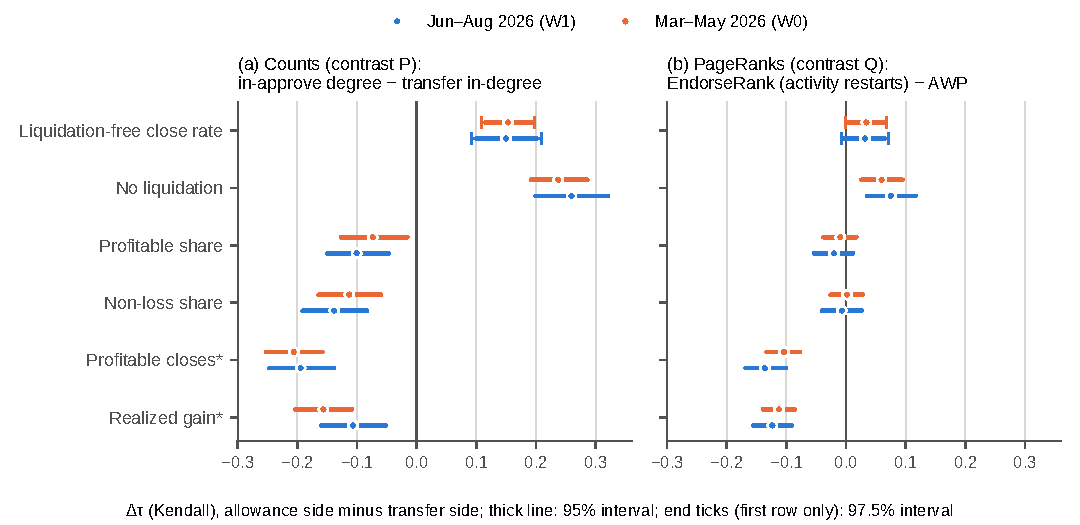
\includegraphics[width=7.2in]{figures/fig_allowance_vs_transfer.pdf}
\end{adjustwidth}
\fi
\caption{{\bf Allowance side minus transfer side on six later trader outcomes, in two windows.}
Each point is a paired difference in Kendall's $\tau_b$ between an allowance-side and a transfer-side score frozen at the start of a three-month label window. Thick lines are unadjusted 95\% paired bootstrap intervals (2,000 resamples). On the first row only, thin lines with end ticks show the 97.5\% intervals; in W1 these are the decision intervals of P and Q, and in W0 they are descriptive. Panel (a): in-approve degree minus transfer in-degree (contrast P). Panel (b): EndorseRank with activity restarts minus AWP, which share edge weights and restart rule and differ only in the edge type (contrast Q). Blue: W1, freeze 31 May 2026, labels June--August 2026 ($n=1{,}402$ traders); its cohorts and labels were registered for a companion study, but the contrasts shown here were not. Orange: W0, freeze 28 February 2026, labels March--May 2026 ($n=1{,}860$). An asterisk marks the two labels that grow with the number of closes. Pre-specified post hoc analysis.}
\label{fig1}
\end{figure}

\textit{Who the recipients are.} The count-level lead rests on few addresses (Table~\ref{tab4}). In W1, 95.5\% of recipients had no liquidation against 42.0\% of other traders, a risk difference of $+0.534$ $[0.459,0.593]$; in W0, 97.4\% against 49.4\% ($+0.481$ $[0.418,0.523]$). Recipients were not simply less active: they closed more positions (median 23 against 16.5 in W1) and had lower mean profitable and non-loss shares (0.347 against 0.456 and 0.435 against 0.668), the pattern behind R3. Most W1 recipients were already W0 recipients, so W0 observes largely the same addresses three months earlier rather than replicating the result on new entities; across both windows the evidence rests on a few dozen distinct addresses, a clustering the wallet bootstrap ignores. Without the ten recipients of highest in-approve degree P remains $+0.124$ $[0.073,0.174]$ in W1 and $+0.133$ $[0.093,0.172]$ in W0, but with nearly all recipients at degree one the ten dropped are effectively arbitrary. Almost every recipient is a contract account: 40 of 44 in W1, with three of unknown type and one EOA, and 38 of 39 in W0, with one EOA. Account type is therefore an unresolved confound of this signal, and one the design cannot assess, since traders without approvals were never classified. One explanation would fit every row of the table: recipients may be vault, hedging or aggregator contracts that others authorize to move their tokens, that trade at low leverage and rebalance often, and so are rarely liquidated, close many partial positions and earn modest profitable shares. The data hold neither leverage nor contract code, so this explanation is untested.

\begin{table}[!ht]
\begin{adjustwidth}{-2.25in}{0in}
\centering
\caption{{\bf Traders that had received an approval at the freeze (recipients) against all other traders.}}
\begin{tabular}{lcccc}
\toprule
 & \multicolumn{2}{c}{W1 (June--August 2026)} & \multicolumn{2}{c}{W0 (March--May 2026)} \\
\cmidrule(lr){2-3}\cmidrule(lr){4-5}
 & Recipients & Other traders & Recipients & Other traders \\
\midrule
Traders & 44 & 1,358 & 39 & 1,821 \\
In-approve degree at the freeze & \multicolumn{2}{l}{1 for 39 recipients, 2 for 5} & \multicolumn{2}{l}{1 for all 39 recipients} \\
Share with no liquidation & 0.955 & 0.420 & 0.974 & 0.494 \\
Mean liquidation-free close rate & 0.986 & 0.865 & 0.997 & 0.888 \\
Mean profitable share & 0.347 & 0.456 & 0.347 & 0.455 \\
Mean non-loss share & 0.435 & 0.668 & 0.398 & 0.647 \\
Median closes in the label window & 23.0 & 16.5 & 27.0 & 15.0 \\
Recipient account types & \multicolumn{2}{l}{40 contract, 3 unknown, 1 EOA} & \multicolumn{2}{l}{38 contract, 1 EOA} \\
\midrule
Risk difference, no liquidation [95\% CI] & \multicolumn{2}{c}{$+0.534$ $[0.459,\,0.593]$} & \multicolumn{2}{c}{$+0.481$ $[0.418,\,0.523]$} \\
P without the 10 top recipients [95\% CI] & \multicolumn{2}{c}{$+0.124$ $[0.073,\,0.174]$} & \multicolumn{2}{c}{$+0.133$ $[0.093,\,0.172]$} \\
\bottomrule
\end{tabular}
\begin{flushleft}Recipients have an in-approve degree above zero at the freeze; most W1 recipients are also W0 recipients. Account types come from the code lookup of the spring spender cohort; a recipient outside that cohort is unknown, and other traders were not classified. EOA: externally owned account. Intervals use the resamples of Table~\ref{tab3} and are unadjusted and descriptive. The last row drops the ten recipients of highest in-approve degree; with tied degrees, which ten are dropped depends on the sort order (see Materials and methods). Pre-specified post hoc analysis.
\end{flushleft}
\label{tab4}
\end{adjustwidth}
\end{table}

\subsection*{Computational cost}

On the same wallets, with the same solver and settings, EndorseRank solved in 0.55\,s and AWP in 5.03\,s (means of five runs, standard deviations 0.014 and 0.062\,s), a time ratio of 9.2 that tracks the edge ratio of 9.3 (14,727 against 137,087 edges). About 94\% of each call is spent assembling the sparse transition matrix, so the speed comes from the sparser graph and not from any algorithmic advantage.

%======================================================================
\section*{Discussion}

\subsection*{The edge matters; on this sample the walk does not}

The two edge types measure different things, and the out-of-window results show it in both windows: scores built on allowances track later approvals, and scores built on transfers track later inflow. Choosing the edge is therefore a decision about what a reputation score is meant to follow, not a technical detail. Propagating along the chosen edge added nothing measurable on the label of the edge's own construct: in each window the raw count ranked that label better than the walk that smooths it, by $0.12$ to $0.32$ in $\tau$. That is unsurprising given preferential attachment and link-prediction practice~\cite{barabasi1999,newman2001,libennowell2007,lin2022linkpred}, but on-chain reputation work rarely tests it, comparing walks with each other or with statistics of their own edges~\cite{do2023awp}. Part of each margin may come from how $\tau_b$ treats a tied count and a nearly tie-free walk, and arrival counts as labels favor any score that tracks the current number of counterparties.

For EndorseRank the closed form shows what the walk computes on this sample. On a depth-one graph every endorser holds the same score, so the walk cannot carry information about who the endorsers are beyond how widely each one approves. What remains is a reweighting of the approval count by time, by token and by each owner's breadth of approval, and on these labels the reweighted count lost to the plain one. The sample never observed longer endorsement paths, so a deeper sample, and labels that are not counts of arrivals, could produce a different answer.

\subsection*{Allowance information and liquidation avoidance}

The trader outcomes are recorded by the exchange and not by either graph. On one of them, later avoidance of forced liquidation, the allowance side ranked traders and the transfer side did not, while transfer-side scores ranked the two outcomes that rise with trading volume. That fits transfer scores recording how much an address trades, as their construction from payments, past payouts from the exchange included, suggests, though we did not measure the link directly.

The limits of this result are part of it, and we state them in full here once.
\begin{itemize}
\item \textit{Timing.} The analysis is pre-specified post hoc, and in W1 the point estimates of P and Q were implied by numbers known when the plan was written; P was chosen with that knowledge.
\item \textit{Independence.} The windows share scoring data and largely the same recipients, so W0 is an earlier look at the same addresses, not a replication, and the effective sample is a few dozen recipient addresses.
\item \textit{Predictor.} Among traders the in-approve degree is an indicator held by about 3\% and 2\% of them, so P mixes rarity with association, and the risk difference describes the effect more directly.
\item \textit{Account type.} Nearly all recipients are contracts, other traders were never classified, and types were read after both windows, so the design cannot separate the signal from account type, which may account for all of it.
\item \textit{Past behavior.} The result was not compared with what a venue already knows before the freeze, such as a trader's own liquidation history, number of closes or leverage, so it shows no value beyond past behavior.
\item \textit{Labels and selection.} Partial closes raise the liquidation-free rate of traders who close in steps; requiring three closes in the label window conditions on later activity and may drop traders wiped out early, perhaps at different rates by recipient status; and the W0 seed cohort was selected on closes inside its own label window.
\item \textit{Construct.} The signal is lower on the profitable share, so it concerns liquidation avoidance, not trading success, and nothing here suggests that approvals measure creditworthiness, default risk or trading skill.
\item \textit{Walks.} The like-for-like PageRank pair points the same way in both windows but is not resolved, so the result does not show that EndorseRank ranks liquidation avoidance better than AWP.
\end{itemize}
\noindent Within these limits, whether allowance information is the better basis for reputation measured on an outcome neither graph contains receives a qualified answer: a provisional yes at the count level and for forced-liquidation avoidance, in a post hoc analysis confined to a few dozen mostly contract accounts and possibly owing to account type; no for trading success; and open at the level of the walks. Whether the signal would help a venue screen counterparties was not tested.

\subsection*{Implications for evaluating on-chain reputation}

The study suggests four practices for evaluating on-chain reputation scores. First, report the raw counts beside every walk: here no walk beat the count of its own edge type on the label of its own construct, and EndorseRank also fell below the approval count on liquidation avoidance under the plan's rule for absent traders, which a walk validated only against statistics of its own edges~\cite{do2023awp} could not have revealed. Second, freeze scores before any label is counted. Third, compare edge types on outcomes that neither was built from, since each leads on the labels of its own construct by design~\cite{cronbach1955}, and check how separate those outcomes really are; even then, which side leads depends on the outcome. Fourth, judge a score against the baseline the decision maker already holds, such as an address's own past outcomes, with statistics whose scale does not depend on ties or prevalence. Committing the comparison to a plan, and stating what was already known, is what makes a post hoc analysis of existing data interpretable~\cite{nosek2018}.

\subsection*{Practical implications}

For operators the results argue for caution more than adoption. The in-approve degree predicted later approvals better than any walk and needs no solver, but as a raw count of distinct owners it is cheaper to inflate than a uniformly restarted PageRank: approvals from $N$ fresh addresses raise it by $N$ for $N$ transaction fees, with no tokens locked. Among traders it is zero for about 97\% and 98\% of addresses in the two windows. Any use of it, or of the liquidation signal, in screening would first need a registered test on new data with account type, past liquidation behavior and leverage controlled. EndorseRank inherits the exposure of uniformly restarted PageRank to farms of addresses that approve one another~\cite{gyongyi2005alliances,cheng2005}, which the companion manuscript quantifies; restarts limited to a vetted seed set, as in TrustRank~\cite{gyongyi2004trustrank}, would bound closed farms but were not tested. For transfer hubs and their inflow, the transfer in-degree is the stronger baseline. None of these scores replaces collateral~\cite{gudgeon2020crisis} or should allocate rewards or credit without controls against Sybil identities~\cite{douceur2002}.

\subsection*{Limitations}

The evidence comes from one chain, one six-month scoring window and two three-month label windows, so other rollups, Layer-1 networks or lending venues would need new data~\cite{werner2022}. Both graphs are one-hop ego networks of a trader cohort. AWP was run with its value weight in effect switched off, and EndorseRank's uniform restart rule was chosen after both rules had been scored. The spender comparisons were not fixed before the spring labels were known, and in W1 EndorseRank was scored after the registered evaluation, so W1 repeats them on later data without registering them. The spender labels are sparse, with 136 to 222 non-zero values each, and concern contracts more than user wallets. Every interval treats wallets as independent and the graphs as fixed, although spenders share owners and recipients may share code, so the intervals are probably too narrow; the spender holdouts use only 400 resamples, and only the decision pair is adjusted for multiplicity. The \texttt{Approval} event can record spends as well as grants, and allowances inside contracts such as Permit2 are unseen (S1 Text). Market conditions, which drive liquidations, were not measured and may have differed between windows; at least one liquidation struck about half of the W0 traders and 56\% of the W1 traders. No default labels from unsecured lending were available, and no causal claim is made.

These limitations define the next steps. For the liquidation result: a registered test on a window not yet extracted, with account types read at the freeze block for every labelled trader and recipient contracts grouped by code; baselines from each trader's pre-freeze liquidation record, closes and leverage, with the incremental value of recipient status estimated in a regression; a position-level liquidation rate and eligibility from one close; the risk difference and a rank statistic that counts ties as one half; and a bootstrap that resamples recipient entities. A 97.5\% interval half-width of about 0.015 for the like-for-like PageRank contrast would resolve a difference of the size seen here. For the spender results: a tie-robust comparison of each walk with its count, and an ablation of the time weights, token weights and owner normalization. Deeper extraction would give a walk something to propagate, and value weights on price-normalized amounts, seed-restricted restarts and the isolated-node rule should be fixed before they are scored.

%======================================================================
\section*{Conclusions}

Authorization edges and payment edges carry different information about the same addresses. On Arbitrum One, scores built on the latest allowances tracked which spenders, most of them contracts, would gain new approvals, and scores built on transfers which would gain new senders. In neither window did PageRank improve on the raw degree of its own edge type on the label of its construct, and on a depth-one graph EndorseRank is a common constant times one plus the damped owner-normalized in-strength, a reweighted approval count with nothing to propagate. Allowance edges carry information that transfer edges do not about later approvals and, in a post hoc analysis confined to a few dozen mostly contract accounts, about later liquidation avoidance. That second signal holds for counts but not, so far, for the like-for-like PageRanks; it may owe to account type, was not compared with traders' own past behavior, and does not extend to trading success. It awaits a registered test with account type and past behavior controlled.

\section*{Acknowledgments}

[Acknowledgments to be completed by the authors.] The use of Claude (Anthropic) in the analysis and in writing is described under Use of generative AI in Materials and methods.

\nolinenumbers

\bibliography{references}

\section*{Supporting information}

\paragraph*{S1 Text.}
\label{S1_Text}
{\bf Event decoding, label formulas and extraction queries.} Contract addresses, topic hashes and decoded fields of the ERC-20 and GMX~V2 events, exact formulas of every spender and trader label, the account-type lookup, the SQL queries, and the properties of the data that were not quantified.

\paragraph*{S1 File.}
\label{S1_File}
{\bf Analysis plan for the trader comparison.} The plan and claim ledger as committed on 9~October~2026 (commit \texttt{20e250f9481e955f7b622a9ecf7b5cafa82951a1}), reproduced verbatim; SHA-256 of the file \texttt{ba731ff2ba5db4e2c10a7e11f0d3b025e291c4883be2e45cc42fdd7b665ac209}.

\paragraph*{S1 Table.}
\label{S1_Table}
{\bf Windows, cohorts, graphs and labels.} Descriptive statistics of both windows, from the seed cohort to the recipients.

\paragraph*{S2 Table.}
\label{S2_Table}
{\bf All contrasts of the pre-specified trader comparison.} Every contrast of the plan on all six trader labels in both windows, with 95\% and 97.5\% intervals, including the three contrasts that involve walks of the companion study and the stratified rows.

\end{document}
